
\section{\name: Input Protection System}
\label{sec:integriKey}

In this section, we present \name, our system for user input integrity protection for remotely configurable safety-critical systems. Our system includes two main components: (1) the embedded trusted device realized as a simple USB bridge that we call for short \device and (2) a server-side user input matching library. To enable easy deployment, we use WebUSB~\cite{webusb}, a recently introduced browser API standard supported by the Chrome browser. This API allows JavaScript code, served from an HTTPS website, to communicate with a USB device, such as our \device. To prevent swapping attacks, we propose a simple \emph{user labeling} scheme where the user is instructed to annotate swappable input values. 
%Later, in Section~\ref{sec:integriTool}, we describe a UI analysis tool that assists developers in deployment of such labeling.

\subsection{Pre-configuration}
\label{sec:integriKey:initialization} 

Our system requires a secure (authenticated, encrypted and replay-protected) channel from the embedded device (\device) to the remote server. In our system, we leverage standard TLS and existing PKIs for this. To enable server authentication, the public key of the used root CA is pre-configured to \device. To enable client authentication, we use TLS client certificates. Each \device device is pre-configured with a client certificate before its deployment to the user, and the server is configured to accept such client certificates. 

Besides input integrity protection, user authentication to the remote server without revealing the user's credential to the compromised host is also important. Our current implementation does not implement such user authentication, but in Section~\ref{sec:discussion} we discuss how this can be enabled.

%\red{More details about the initialization process: offline vs online, client certificate signed by the device maker}


\subsection{System Operation}

%
% System figure for next section
%
\begin{figure*}[t]
 \centering
  %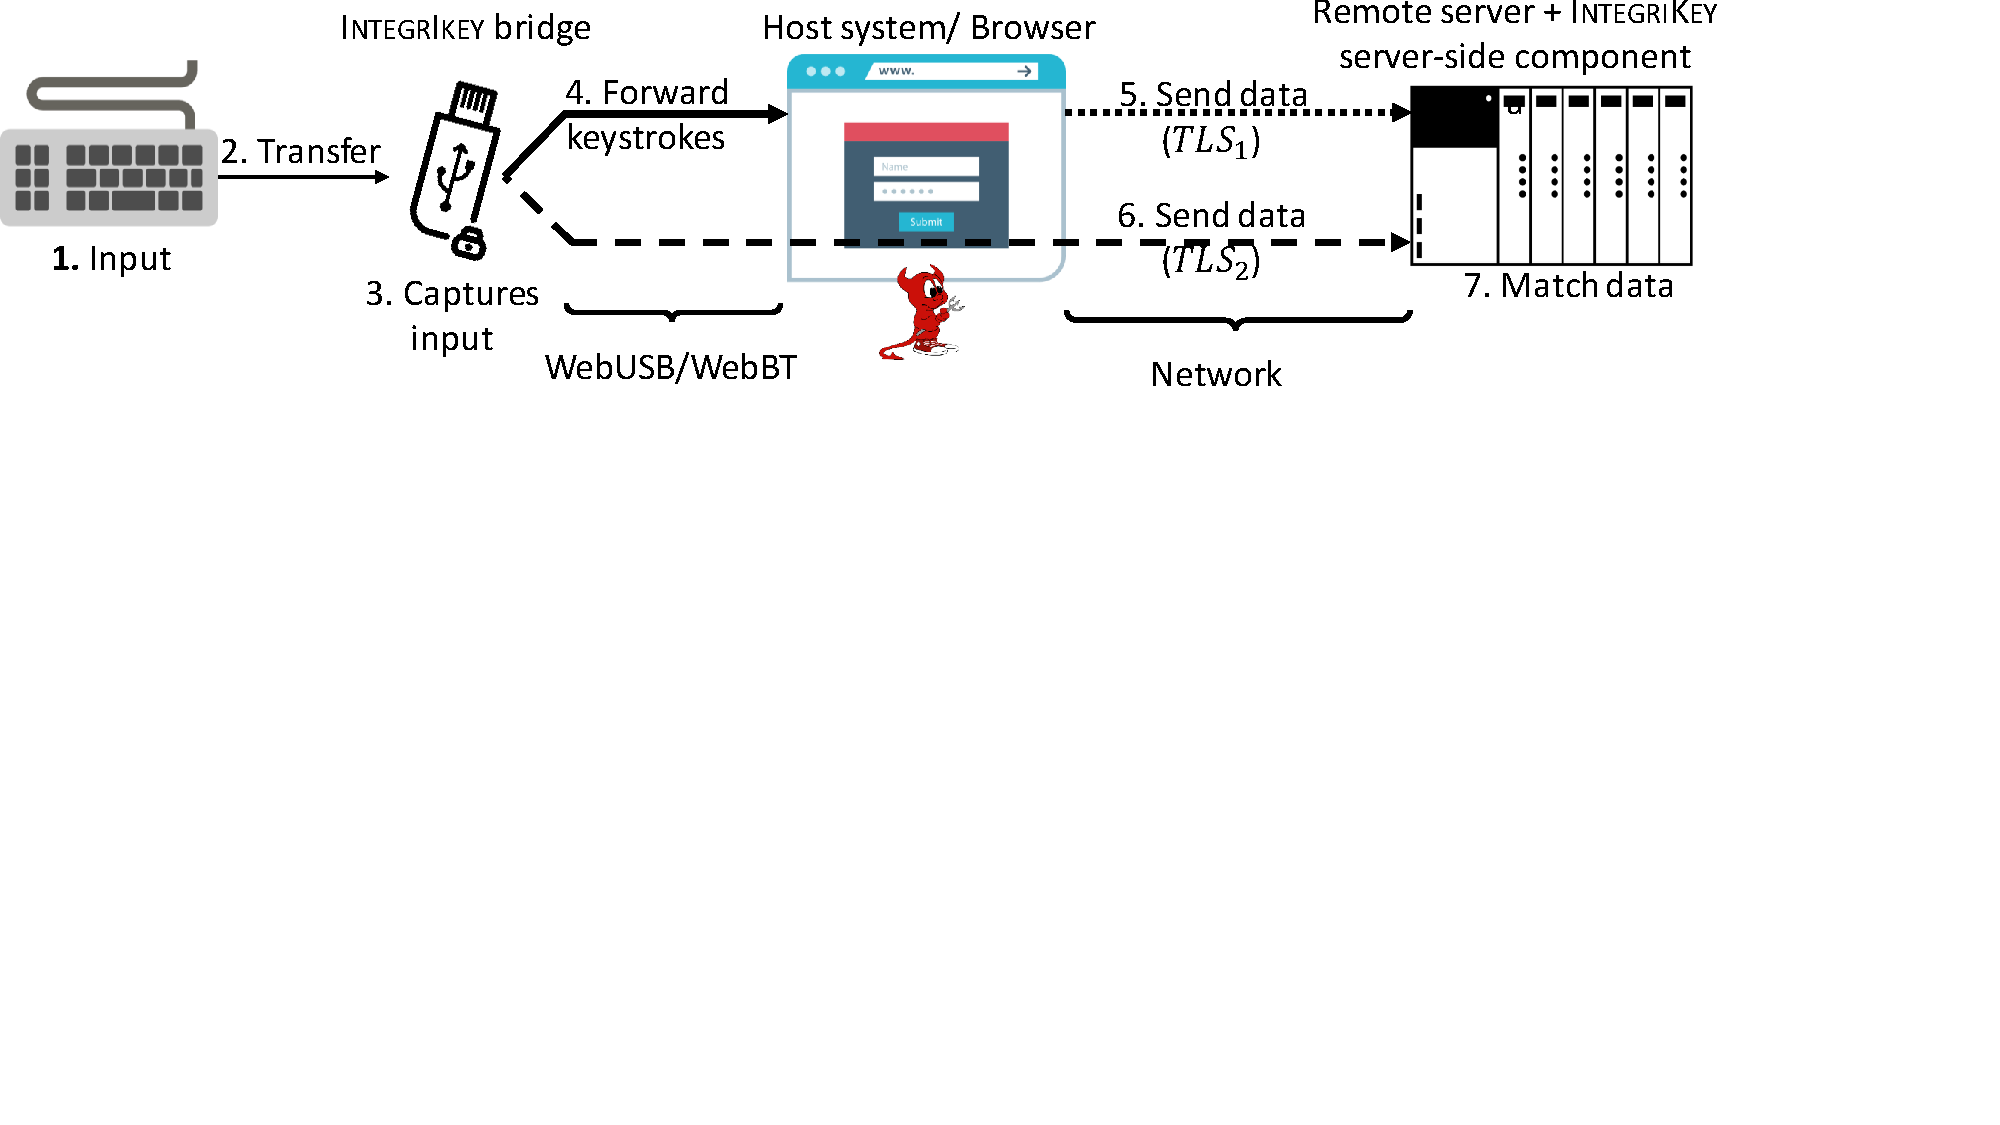
\includegraphics[trim={0 11cm 4.5cm 0},clip,width=0.9\linewidth]{SystemDesign_forms_revised_3.pdf}
  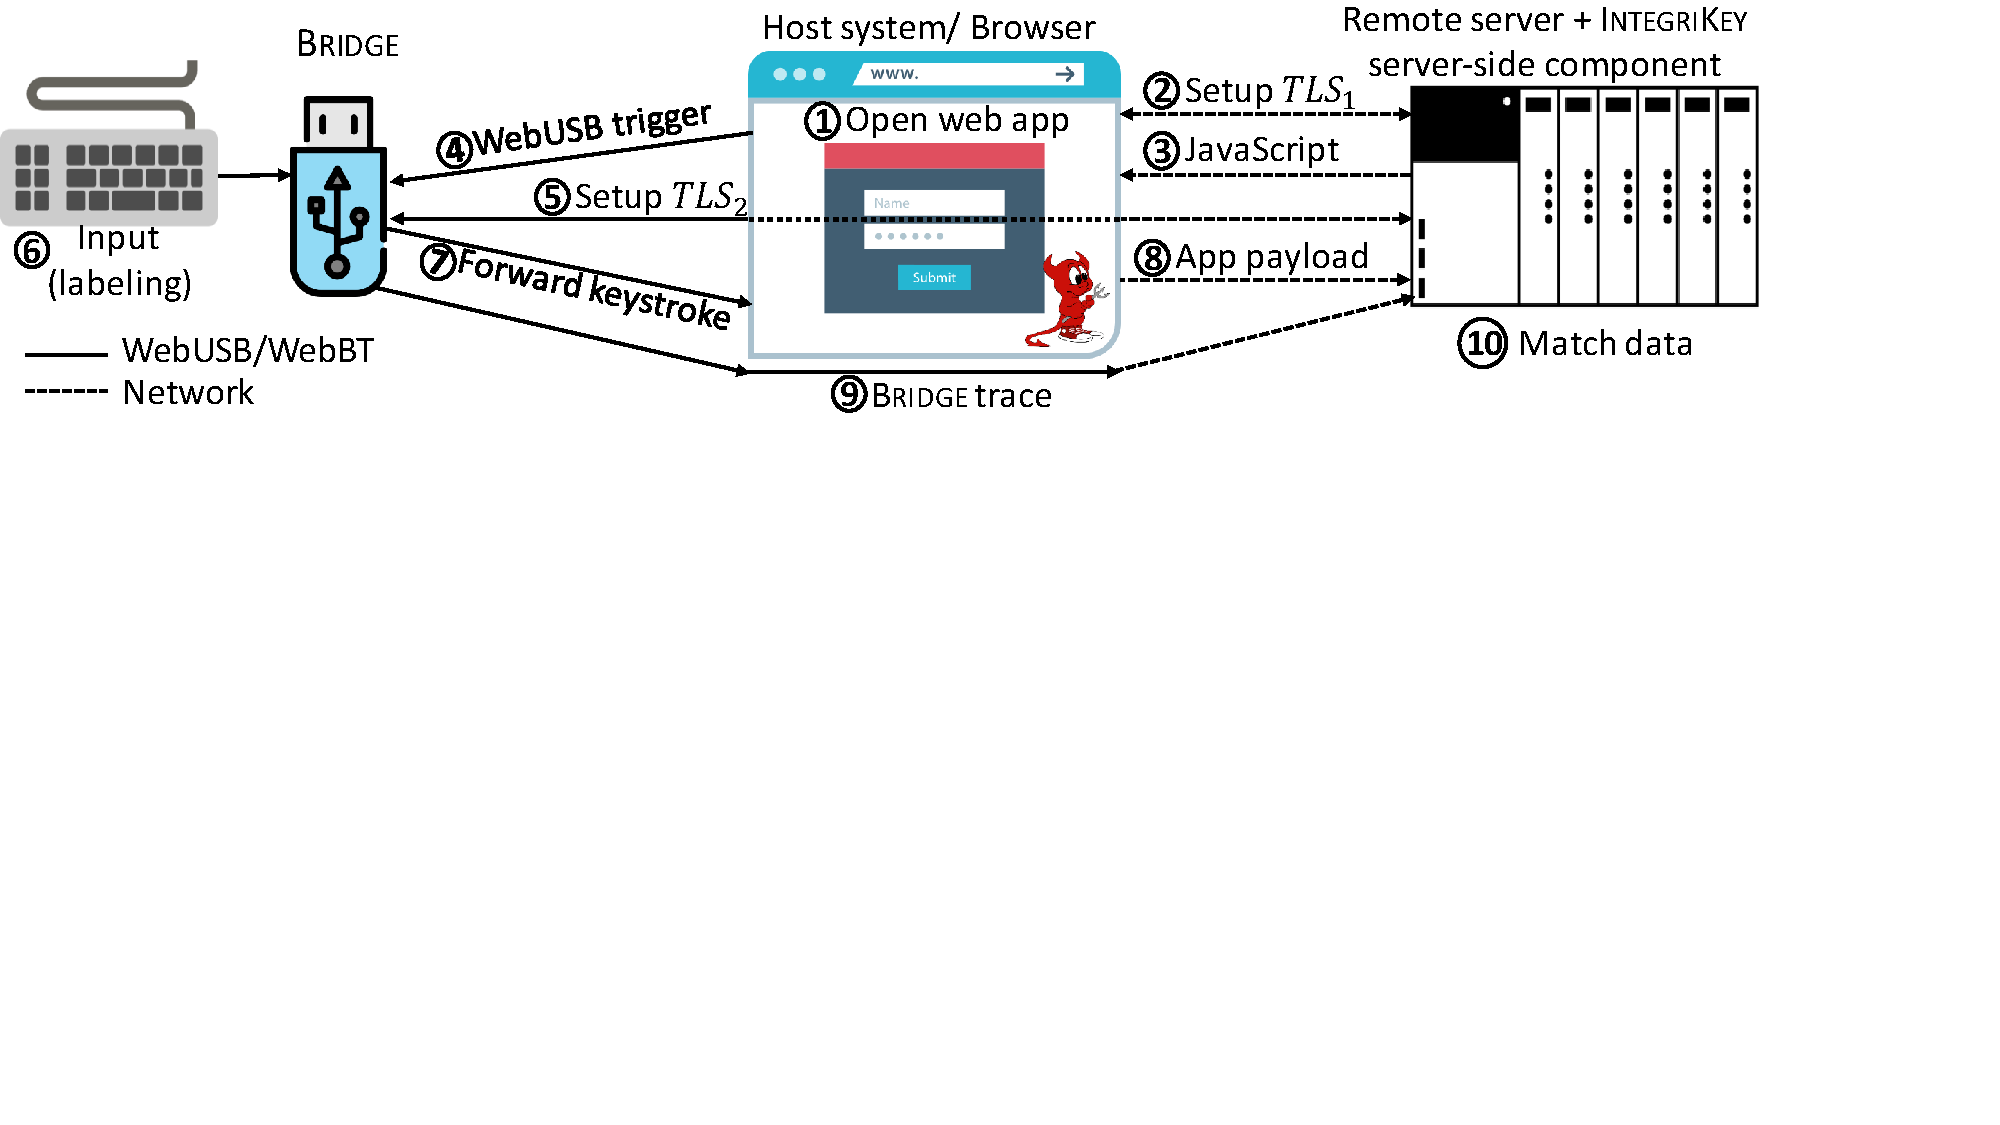
\includegraphics[trim={0 11cm 4cm 0},clip,width=0.95\linewidth]{chapters/IntegriKey/images/SystemDesign_forms_revised_5.pdf}
 \caption[\name operation]{\textbf{\name operation}. The browser on the host opens a standard TLS connection ($TLS_1$) to the server which replies with a web page and JavaScript code. Using the WebUSB API, the JavaScript code invokes the \device that will establish another TLS connection ($TLS_2$) to the server. The \device forwards received keystroke events to the host and periodically sends a trace of them to the server that performs matching between the traces and the received application payload.}
 \label{fig:systemDesignForms}
\end{figure*}

Next, we describe the operation of the \name system that is illustrated in Figure~\ref{fig:systemDesignForms}. 

\begin{enumerate}
    \item The user attaches the \device device between the host and the keyboard. The user starts the browser on the host and opens the web page for remote configuration of the target safety-critical device. 

    \item The browser establishes a server-authenticated TLS connection ($TLS_1$) to the server. 
    %\todo{User authentication discussed elsewhere separately?}

    \item The server sends the web configuration form to the browser together with JavaScript code. The web form includes instructions for user labeling, as described below in Section~\ref{sec:integriKey:labeling}.
    
    \item The browser shows the web form to the user and runs the received JavaScript code that invokes the \webusb API to communicate with \device. The browser passes the server URL to \device.

    \item Based on the received URL and the pre-configured trust root and client certificate, \device establishes a mutually-authenticated \tls connection ($TLS_2$) to the server through the host using the WebUSB API. Mutually-authenticated TLS 

    \item The user completes the web form, as explained in Section~\ref{sec:integriKey:labeling}.
    
    \item \device captures keystrokes and forwards them to the browser.
    
    \item Once the user has completed the web form, the browser constructs a payload (HTTP response) and sends this to the server over the $TLS_1$ connection.
    
    \item \device collects intercepted keystrokes and periodically (e.g., when receiving a tab or return key press, or on every keyboard event) sends a trace of them to the server through the $TLS_2$ connection. 

    \item The server compares the received application payload and traces (input trace matching), as explained in Section~\ref{sec:integriKey:server}. If no mismatch is detected, the server accepts the received user input. The user can remove \device from the host.
\end{enumerate}

\myparagraph{Handling multiple sessions/tabs} The \webusb driver only allows one browser window to communicate with a \usb device at a time. This restricts the \device to operate on multiple browser tabs or session at the same time. As \name is targeted towards protection of specific security-critical web-based transactions (PLC configuration, payment) as opposed to generic input protection for all web browsing, we do not consider this a problem in practice.

\myparagraph{Handing of key strokes}
%\label{sec:integriKey:handleKey}
The \device acts as a \usb host and handles all keyboard events from the user that includes modifiers such as \texttt{shift}, \texttt{ctrl}, navigation keys, character removal keys such as \texttt{backspace} and \texttt{del} etc. The \device registered itself as a generic \usb plug-and-play device and emulates a keyboard. Hence, the \device replicates all the user keyboard actions and send the them to the browser along with the signed actions (traces) to the server. 
%
As one concrete example, assume that the user types \texttt{shift} + a, b, c and \texttt{backspace}, which appears as \texttt{Ab} in the browser. The \device records the trace as \texttt{[shift + a]+b+c+backspace} and translate to \texttt{A+b} which is received by the remote server. 
\subsection{User Labeling}
\label{sec:integriKey:labeling}

\begin{figure}[t]
 \centering
 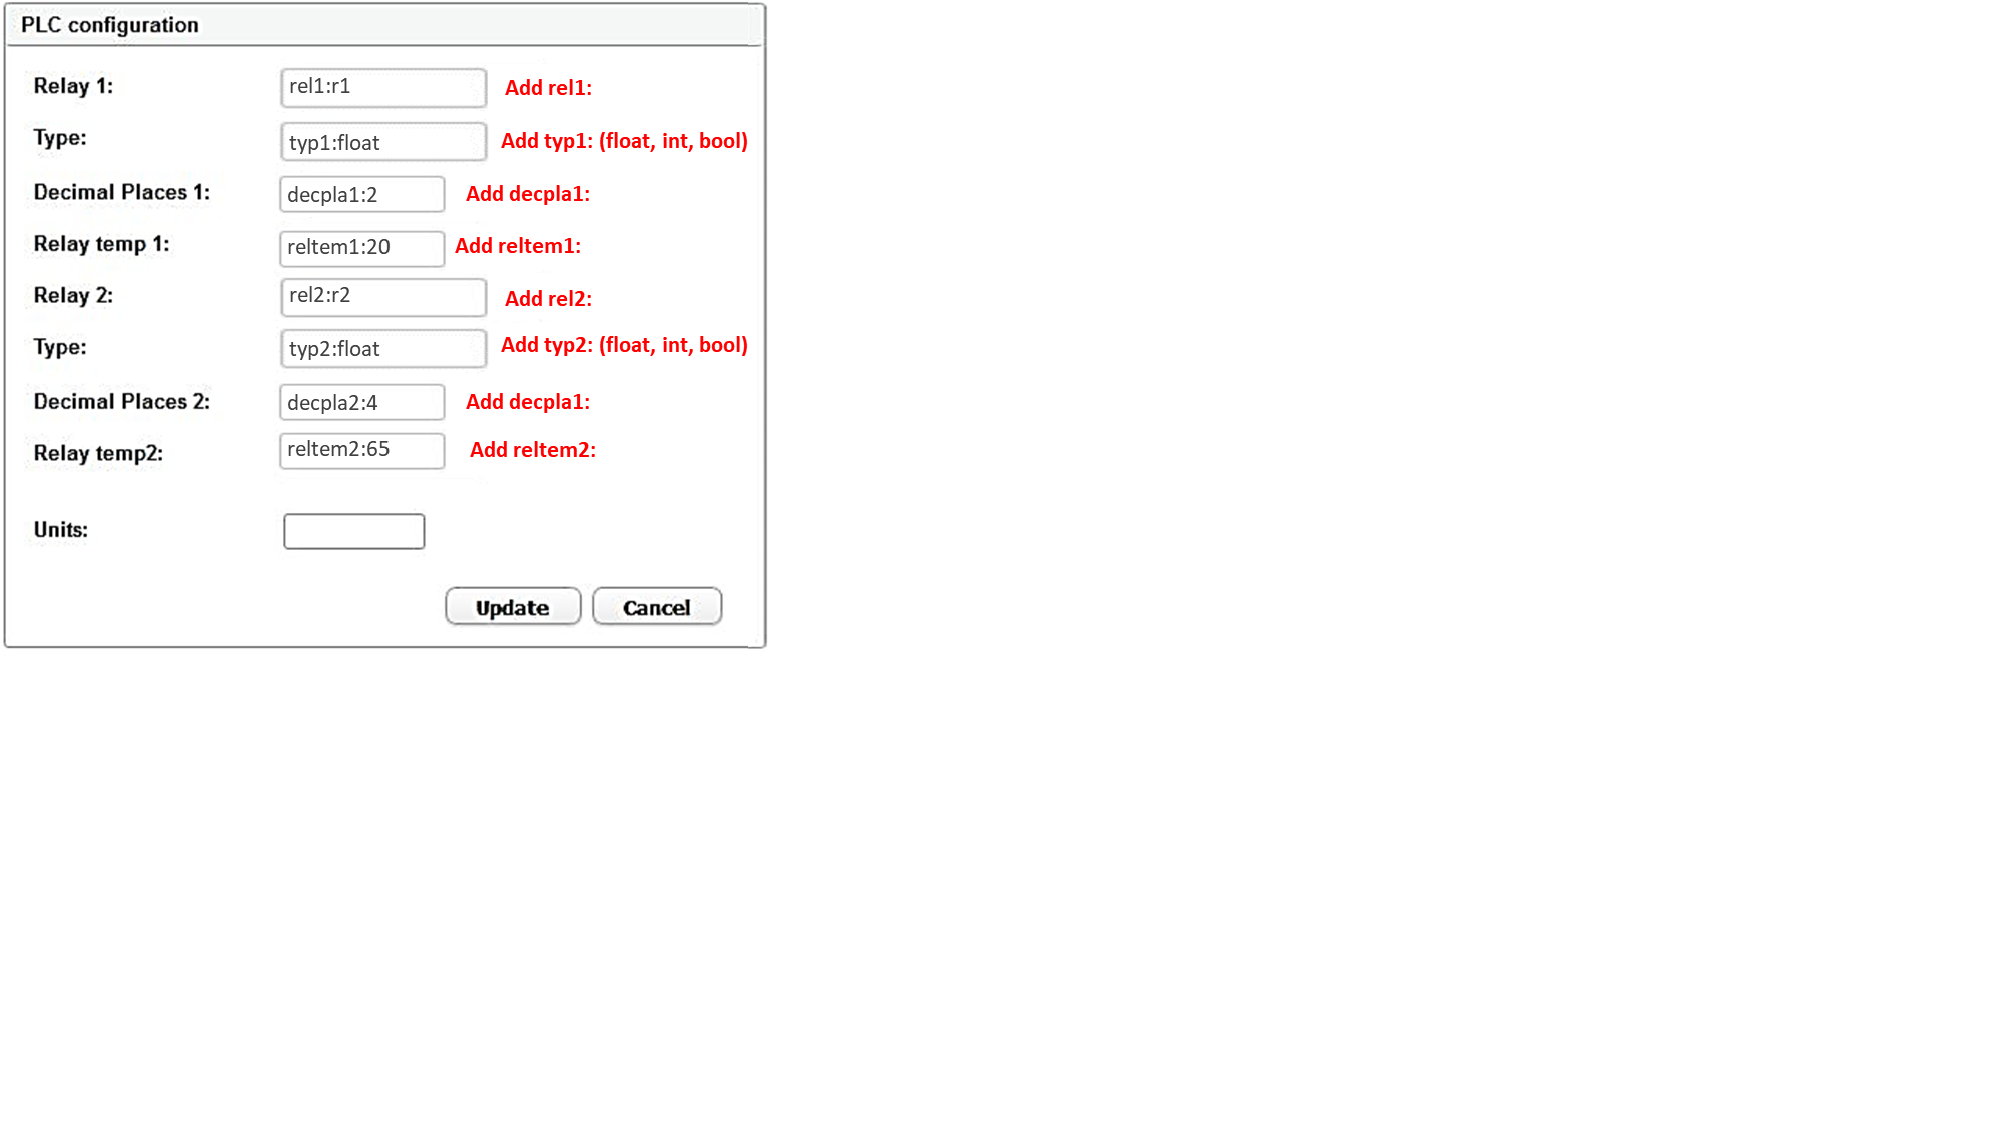
\includegraphics[trim={0 7cm 20cm 0},clip,width=0.65\linewidth]{chapters/IntegriKey/images/labelExample_revised.pdf}
 \caption[User labeling example]{\textbf{User labeling example.} All input fields that need protection against swapping attacks are marked with labeling instructions. For example, to enter a value 20 to the input field \texttt{`Relay temp 1'} the user should type in \texttt{`reltem1:20'} as indicated in the web form next to the input field.} 
 \vspace{-10pt}
 \label{fig:labelEx}
\end{figure}

To prevent swapping attacks explained in Section~\ref{sec:ourApproach:challenges}, we introduce a simple user labeling scheme. In this scheme, the user is instructed to annotate each interchangeable input with a textual label that adds \emph{semantics} to the input event traces and thus allows the server to detect user input manipulation like swapping attacks.

An example of the user labeling process is illustrated in Figure~\ref{fig:labelEx}. When the server constructs the web form, it adds labeling instructions to it. These instructions indicate the textual label, such as \texttt{`rel1:'} for input field named \texttt{`Relay 1'}, that the user should type in. The server adds such labeling instructions to each input field that needs protection against swapping attacks. In Section~\ref{sec:integriTool} we explain an automated UI analysis tool that helps the developer to securely find all such input fields and update the UI accordingly.

For each such field, the user types in the label followed by the actual input value. For example, to enter value \texttt{'r1'} to the input field with name \texttt{`Relay 1'}, the user types in \texttt{`rel1:r1'}. Some input fields may not require labeling. For example, the \texttt{`Units'} field in our example user interface (Figure~\ref{fig:labelEx}) does not have to be labeled by the user as it is not swappable with any other field.

We consider trained professionals that configure industrial control systems, medical devices, etc. as the primary users of our solution. Such users can receive prior or periodic training for the above-described labeling process. The secondary target group is people such as home automation system owners. In this case, no prior training can be assumed, but the UI can provide labeling instructions.


\iffalse
\begin{figure}[t]
 \centering
 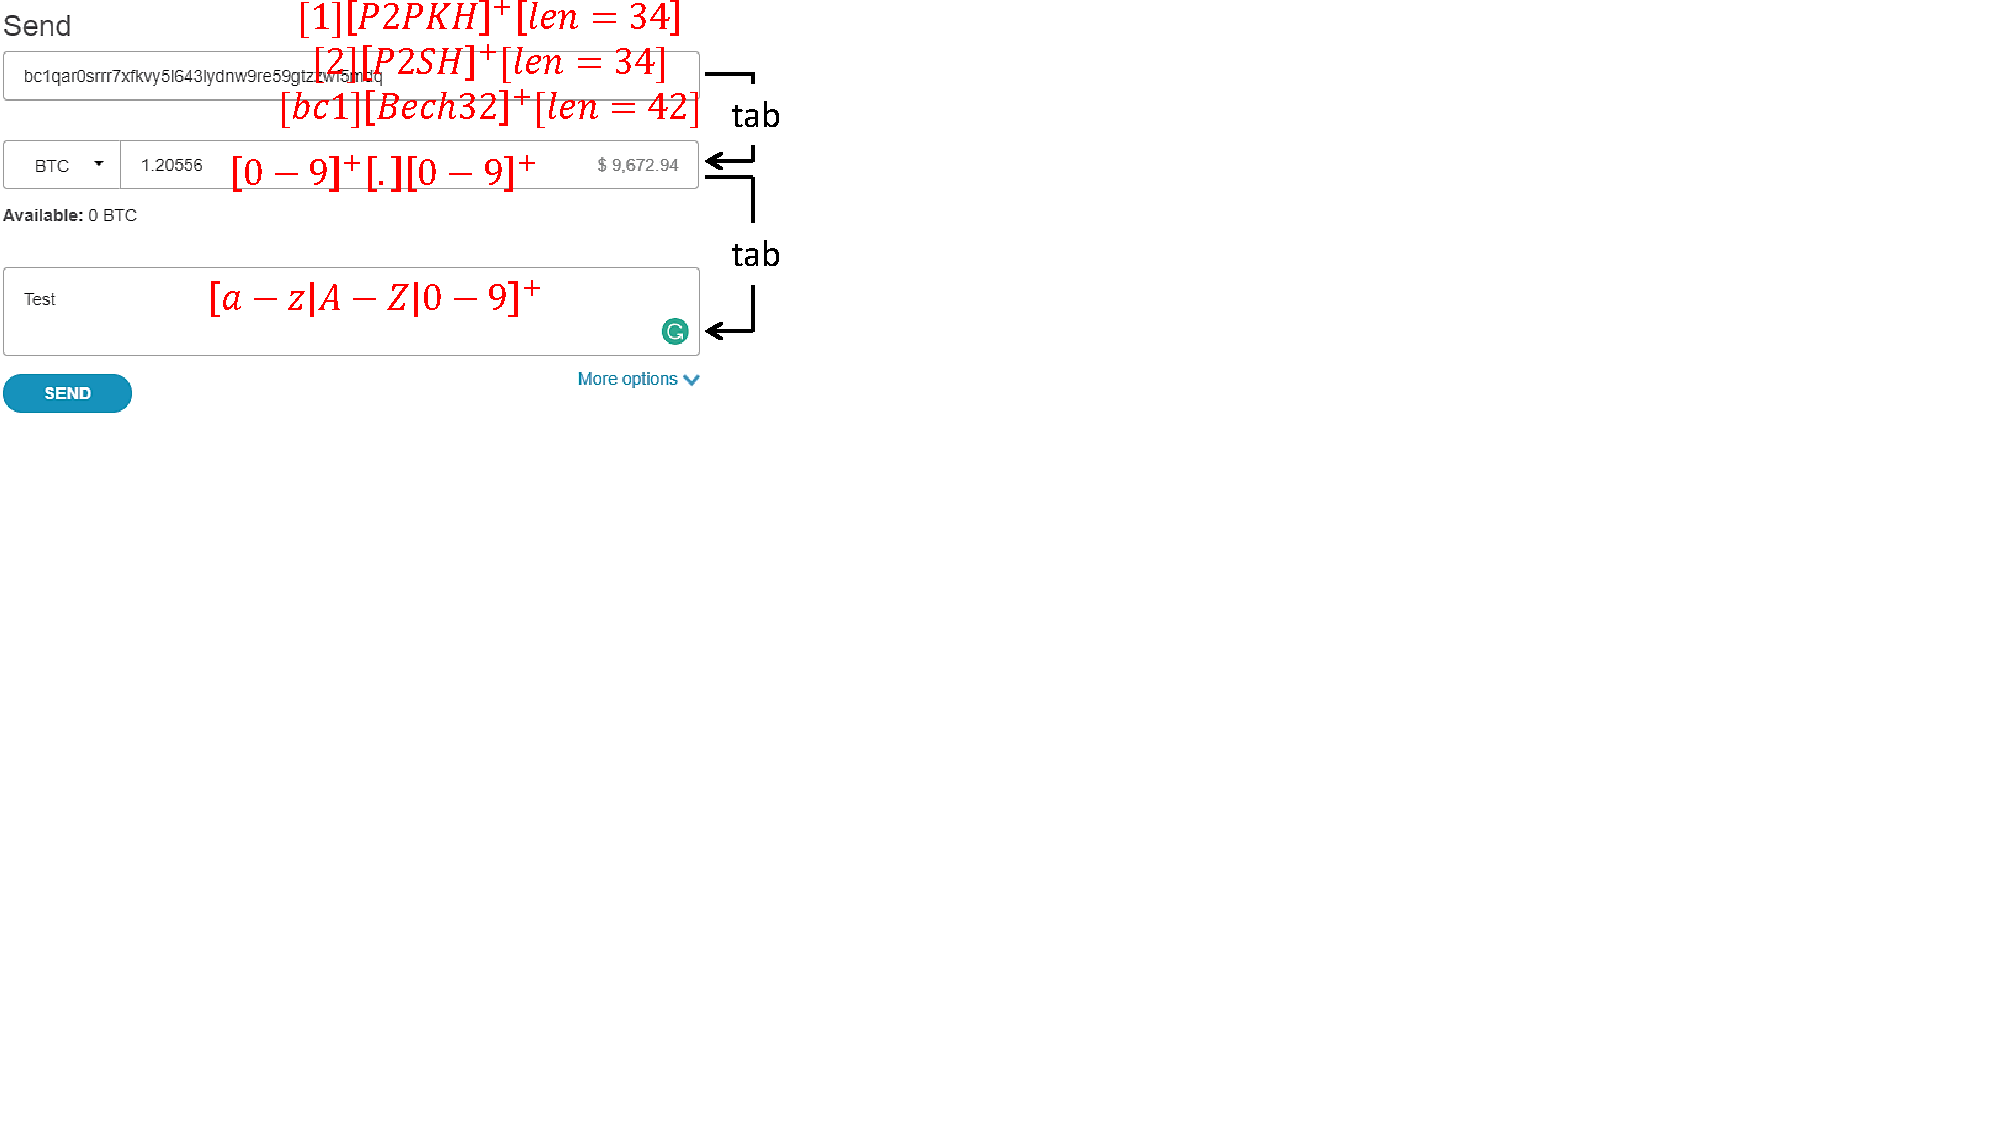
\includegraphics[trim={0 12cm 20cm 0},clip,width=0.8\linewidth]{chapters/IntegriKey/images/InputClassify.pdf}
 \caption{\textbf{Input fields classification.} The \device classifies user input from the specifications received from the remote server.} \vspace{-20pt}
 \label{fig:inputClassification}
\end{figure}

\subsection{Classification of Input Data}

\ad{\#new}
Apart from safety-critical devices such as PLCs and medical devices, \name can be employed in a wide range of applications where input data is sensitive. In such cases, \device classifies the input data to ease the user from labeling them. The specification of the input form (regular expressions) is kept at the remote server's side. When the \device connects with the remote server (more details on the server-side specification in Section~\ref{sec:integriTool:specification}), the server sends the specification to the \device. One such example is email address that has regular expression: $[a-zA-Z0-9.]^*[a-zA-Z0-9]^*$. As the user provides her input through the \device to the browser, the \device intercepts the input signals and do regular expression verification to classify the type of the input. Upon successfully classify the input data, the \device sends the data and the corresponding label directly to the remote server over the dedicated \tls channel between the \device and the remote server.

\myparagraph{Detection of activity} \name provides real-time detection of activity by i) the \device communicating with the remote server and getting the web page context information, and ii) intercepting keystrokes from the users and using the specification of the input to determine the type of input. Figure~\ref{fig:inputClassification} illustrates the input classification on the BitGo web-based wallet bitcoin transaction page. Note that the page contains 3 fields namely the address, BTC amount and a transaction reference field. The figure also annotates the specification of the corresponding fields. The \device intercepts the keyboard input from the user and determine which type of input it is by tallying it to the corresponding specification. The \texttt{tab} input from the keyboard signals the \device that the user changes the input fields.  
\fi

\subsection{Server Verification}
\label{sec:integriKey:server} 

To verify the integrity of the received user input, the server performs a matching operation shown in Figure~\ref{fig:payload}. 

\begin{figure}[t]
 \centering
 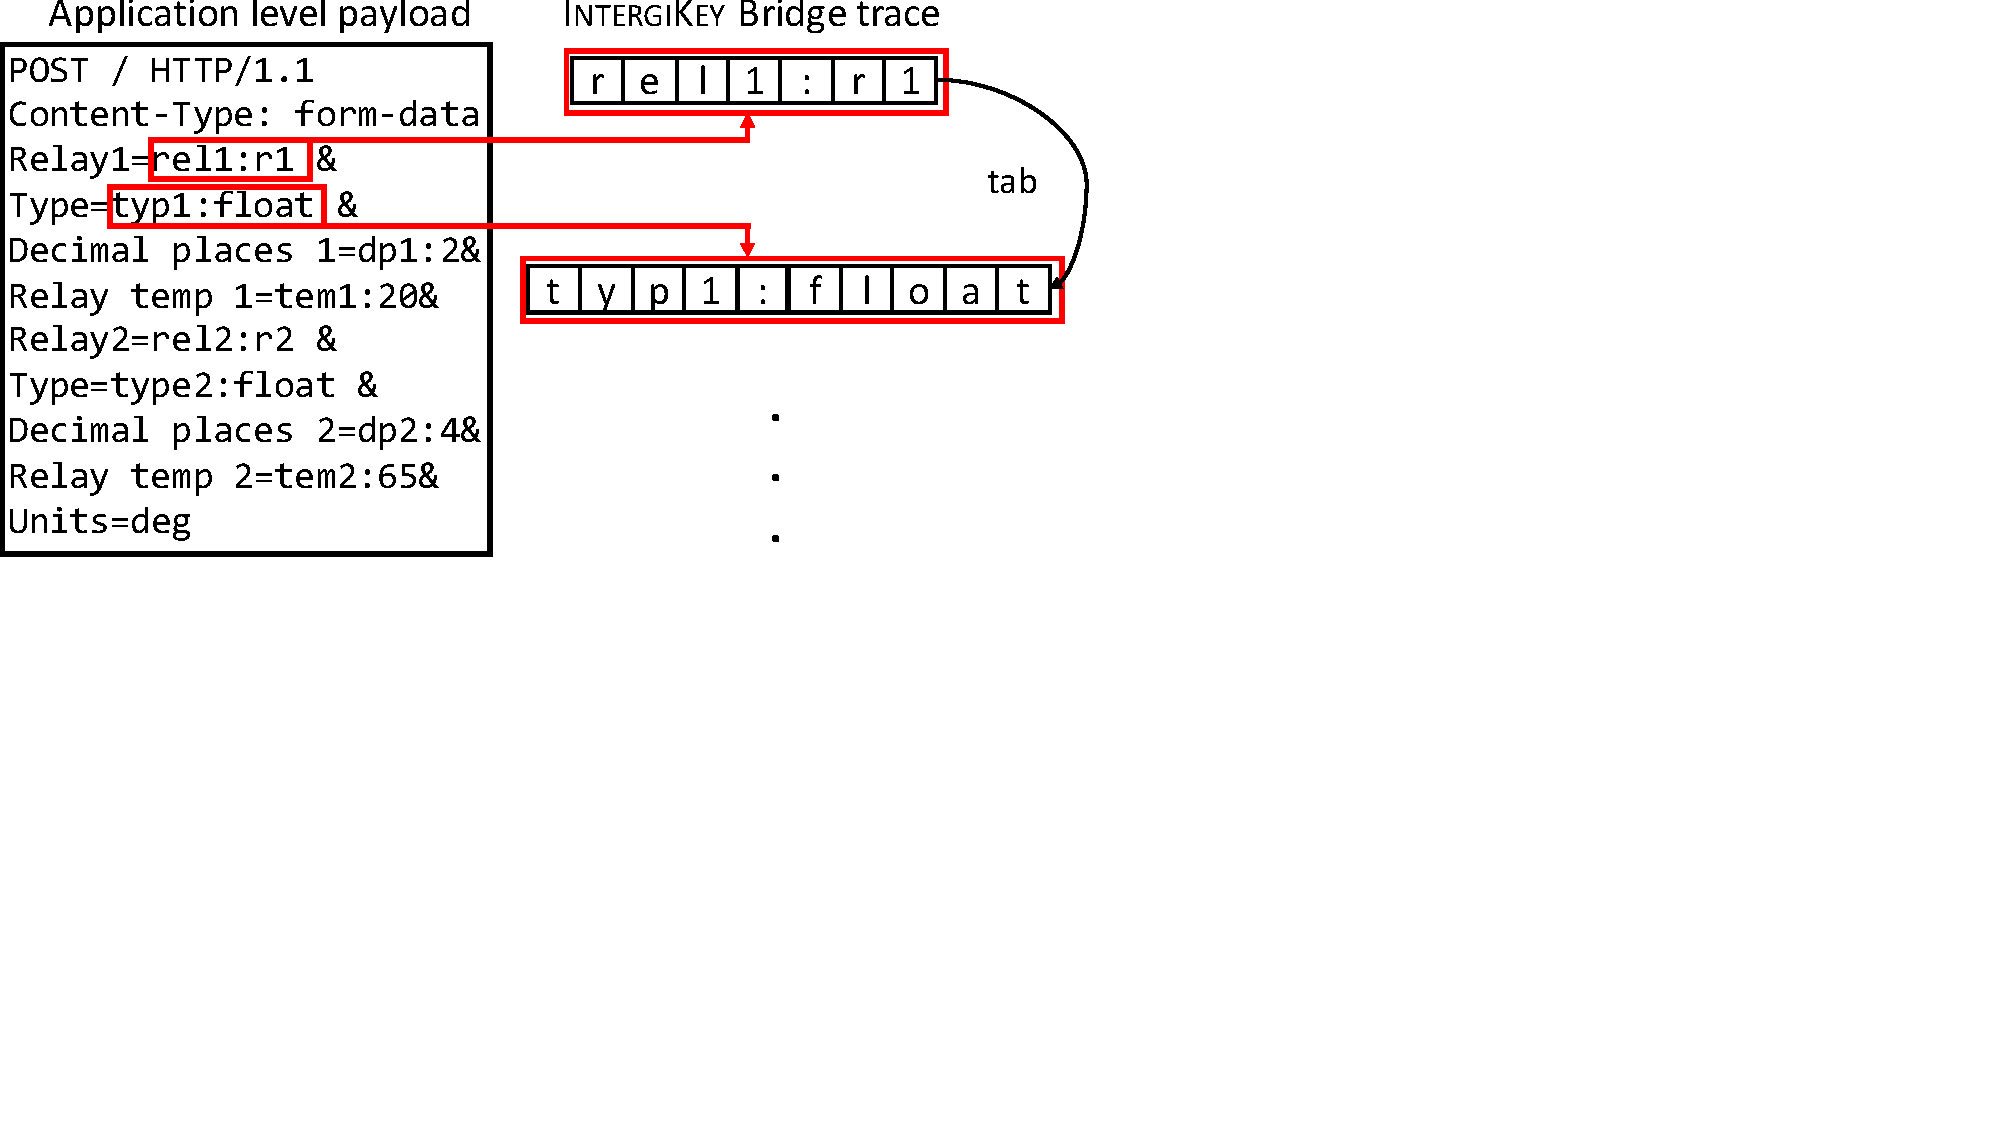
\includegraphics[trim={0 8cm 15cm 0},clip,width=0.8\linewidth]{chapters/IntegriKey/images/FieldPayload_revised_1.pdf}
 \caption[Input trace matching]{\textbf{Input trace matching.} The server compares user input values (and their labels) in the application payload (e.g., HTTP POST data) against the user input in the received traces.} \vspace{-10pt}
 \label{fig:payload}
\end{figure}


\myparagraph{Labeled inputs} First, the server parses through the application payload, and for every user input field that requires labeling makes the following checks: the server verifies that (i) the input appears in the expected position in the application payload, (ii) the input has the expected label, and (iii) one of the received input traces contains a matching labeled value. The order in which the correctly labeled value appears in the traces is not a reason for input rejection. For example, in Figure~\ref{fig:payload} the input labeled as \texttt{`rel1'} appears before the input labeled as \texttt{`typ1'}, but also the opposite order in the trace would be acceptable. Such a case might happen, if the user would fill in the web form values in an order that differs from the default top-to-bottom form filling.

\myparagraph{Unlabeled inputs} Next, the server parses through the application payload again, and for every user input field that does not require labeling it performs the following checks: the server verifies that (i) the input appears in the expected position in the payload and (ii) one of the input traces contains the matching value. Also, unlabeled input values can appear in any order the in traces.

%% Previous server-side verification text %%

%For a specific web page with a set of $n$ input fields $\{f_1, f_2, \ldots, f_n\}$, the server expects to receive $n$ inputs via the \https payload when the user submits the form. In this form, only the overlapping fields require the label of the field to be added to the data. The rest do not require the label as they have the distinct specification. The detailed description of how \tool determine the set of overlapping text fields is provided in Section~\ref{sec:integriTool}. 

%Figure~\ref{fig:payload} illustrates the data received from the \device via the dedicated \tls channel and from the browser via the \http connection. These fields correspond to the example configuration web page that we extracted from the \emph{ContolByWeb x600m} IO server in Figure~\ref{fig:PLC}. The server expects that the user provides the label information for the fields \texttt{Relay 1} and \texttt{Relay 2} as these are swappable and also for the group of fields \texttt{Decimal places 1}, \texttt{Decimal places 2}, \texttt{temp relay 1} and  \texttt{temp relay 2}. As the field \texttt{Unit} is a distinct field, the server does not expect a label added to the data as the field is not swappable with any other field. Additionally, the server also receives the signed data from the \device (via the dedicated \tls channel) for verification. Upon receiving the data, the server executes the following steps:

%First the server checks the number of field data corresponding to the webpage. If it matches with the number of input from the \device, the server proceeds to the next step. There may exist some optional fields that are not required to be filled by the user. After that, the server matches the data from the browser (\https) and the \device (\tls) and executes the signature verification. If they match, the server proceeds to the next step. Otherwise, it rejects the data and sends a feedback to the \device. Upon successful matching of the data received from the browser and the \device, the server searches for the input field labels that are added to the data. When found, the server splits the data from the label and parses it. After parsing, the server checks if the data satisfies the specification that is provided to the tool (by matching the data with the regular expression and value/length constraint in the specification). In case the server does not find the label with the data for the overlapping fields, it rejects the data.

\iffalse
\subsection{Hardware-assisted Secure Autofill}
\label{sec:integriKey:autofill}

\ad{\#new}
\device also acts as a hardware-assisted autofill, eliminating the need for storing sensitive data such as user credentials, credit card number, etc. on the browser storage on the untrusted host system. The \device uses its internal flash storage to keep a key-value pairing of the identifier of the input fields and the actual data. The autofill operation is performed by the remote server to send the specific identifier of the input fields to the \device over the \tls channel between the \device and the remote server. \name autofill has two phases: 
\begin{mylist}
\item \textbf{Initialization} step is necessary when the user is providing data to the web application for the first time. The flow of operation is identical to the standard \name operation described previously. The remote server sends the identifiers of the input fields to the \device. The \device stores the user data on its internal flash storage corresponding to the identifier.
\item \textbf{Autofill} phase allows the \device to populate the web forms in the browser from the data that are stored on its flash storage. The remote server achieves this by sending the identifier to the \device over the dedicated \tls channel.
\end{mylist}
\fi


